\section{Implementierung und Integration des Schwellwertschemas}

\label{sec_impl_threshold}

In diesem Abschnitt wird zuerst die entwickelte Bibliothek zur Nutzung eines kryptographischen Schwellwertschemas dargetsellt und anschließend ihre Nutzung in den unterschiedlichen Systemkomponenten beschrieben.

\subsection{ThresholdCrypto \glqq Lib\grqq{}}

%- Bibliothek, die statuslos in allen Teilen des Systems verwendet werden kann.
%
%- Interface

Um die Funktionen des Schwellwertschema unterschiedlichen Systemteilen einfach zur Verfügung zu stellen, wurde eine Bibliothek entwickelt, die in den verschiedenen Komponenten genutzt werden kann. Das öffentliche Interface der Bibliothek stellt folgende Funktionen bereit:

\begin{itemize}
  \item \textbf{Parametergenerierung: } Diese Funktion dient dem Erhalt der benötigten sicheren Primzahl bzw. des Generator (vgl. \todo{ergänzen}). Hierbei kann zwischen Neugenerierung und Verwendung vorberechneter Parameter verschiedener Schlüsselstärken entschieden werden. Näheres dazu ist im Unterabschnitt \textit{Parametegenerierung} zu finden.
  \item \textbf{Schlüssel- und Sharegenerierung: } Durch diese Funktion wird ein zufälliger geheimer Schlüssel erzeugt und aus ihm der öffentliche Schlüssel sowie die einzelnen \textit{Shares} erzeugt. 
  \item \textbf{Verschlüsselung einer Nachricht: } Diese Funktion verschlüsselt mithilfe des öffentlichen Schlüssels eine Nachricht (siehe auch Unterabschnitt \textit{Hybride Kryptographie}). Sie wird im Proxy verwendet.
  \item \textbf{Berechnung einer partiellen Entchlüsselung: } Mithilfe eines \textit{Shares} wird die zugehörige partielle Entschlüsselung einer verschlüsselten Nachricht berechnet. Diese Funktion wird in den Threshold-Clients genutzt.
  \item \textbf{Kombinieren von partiellen Entschlüsselungen: } Aus ausreichend partiellen Entschlüsselungen kann die Nachricht wiederhergestellt bzw. entschlüsselt werden (siehe wiederum Unterabschnitt \textit{Hybride Kryptographie}).
\end{itemize}

Neben den Funktionen werden noch einige Klassen zur Verfügung gestellt, die das Arbeiten mit den Ergebnissen der Funktionen erleichtern sowie Funktionalität wie Serialisierbarkeit ermöglichen:

\begin{itemize}
  \item \textbf{ThresholdParameters: } Enthalten die Werte \(t\) und \(n\) des Schwellwertschemas.
  \item \textbf{KeyParameters: } Enthalten die benötigten Primzahlen bzw. den Generator der zugrundeliegenden Gruppe.
  \item \textbf{PublicKey: } Enthält den öffentlichen Schlüssel der zum Verschlüsseln einer Nachricht verwendet werden kann.
  \item \textbf{KeyShare: } Enthält die Werte des Shares eines Teilnehmers am Schwellwertschema.
  \item \textbf{EncryptedMessage: } Enthält die Daten einer verschlüsselten Nachricht (vgl. auch Abschnitt \ref{sec_impl_threshold_hybrid}).
  \item \textbf{PartialDecryption: } Enthält die zu einer partiellen Entschlüsselung gehörenden Werte, die zum Entschlüsseln der vollständigen Nachricht genutzt werden.
\end{itemize}

Im Folgenden soll kurz auf zwei Kernelemente des implementierten Verfahrens eingegangen werden.

\subsubsection{Parametergenerierung}
  
 \label{sec_impl_threshold_keyparams}
  
%  - Verwendete Gruppen und Auswirkungen fester Parameter? HoC, ...

% https://crypto.stackexchange.com/questions/1451/elgamal-multiplicative-cyclic-group-and-key-generation
% Introduction to modern cryptography 8.3.3 (pdf 343ff)
% Sharing of parameters: Introduction to modern cryptography ElGamal implementation issues (pdf 425)

Die für das Verfahren benötigten sicheren Primzahlen \(p\) und \(q\) lassen sich mithilfe eines einfachen Ansatzes finden \cite{hoc1996}: Es wird solange eine Primzahl \(q\) im Bereich der vorgegebenen Schlüsselstärke zufällig gewählt, bis \(2q + 1\) ebenfalls eine Primzahl ist. Zur Überprüfung der Primalität der entsprechenden Zahlen wird der Miller-Rabin-Test\footnote{
  Der Miller-Rabin-Primzahltest ist ein Algorithmus, der basierend auf probabilistischen Annahmen die Primalität einer Zahl mit durch Angabe von einer Rundenzahl beliebig hoher Wahrscheinlichkeit bestätigen kann.
} genutzt.

Zusätzlich benötigt das Verfahren einen Generator \(g\) einer Untergruppe der Ordnung \(q\) von \(\mathbb{Z}_p^*\). Hierzu wird lediglich solange ein zufälliges Element \(g\) aus \(\mathbb{Z}_p^*\) gewählt bis 

\[g^q \equiv 1 \mod p \text{ und } g^2 \not\equiv 1 \mod p\] 

gelten. Da Untergruppen von \(\mathbb{Z}_p^*\) nach dem Satz von Lagrange lediglich die Ordnungen \(1, 2, q\) oder \(2q\) besitzen, werden durch obenstehende Bedingungen lediglich Untergruppen der Ordnung \(q\) zugelassen.

Nach \cite{katz2014} beeinträchtigt es nicht die Sicherheit des ElGamal-Verfahrens, wenn vorberechnete Parameter von verschiedenen Benutzern geteilt werden. Auch die Kombination dieses Verfahrens mit Shamirs Secret Sharing dürfte hieran nichts ändern, da das Secret Sharing lediglich für die Aufteilung des geheimen Schlüssels in Shares sorgt, aber an den grundlegenden Eigenschaften der Ver- und Entschlüsselung im ElGamal-Schema nichts ändert. Daher wurden verschiedene Parameter bereits vorberechnet und als statische Parameter zur Verfügung gestellt. Weiterhin ist es jedoch auch möglich eigene Parameter in gewünschter Stärke zu generieren. \todo{evtl. auf Evaluation beziehen.} In den meisten Empfehlungen werden heutzutage Schlüssellängen um 2000 Bit empfohlen\footnote{
  Für einen Vergleich verschiedener Empfehlungen siehe: https://www.keylength.com
}.

\subsubsection{Hybride Kryptographie}

\label{sec_impl_threshold_hybrid}
  
%  - Erzeugung symmetrischer Schlüssel und symmetrische Kryptographie per NaCl(pynacl) -> Authenticated Encryption ChaCha Salsa
%  
%  - lediglich Verschlüsselung dieses Schlüssels mit dem Schwellwertschema
%  
%  - von erfahrenen Kryptographen entwickelt
%  - getestet
%  - schnell
%  - Beliebiger Nachrichteninhalt ohne Auswirkungen auf die Verschlüsselung

Die Verschlüsselung bzw. Entschlüsselung wurden in Form eines hybriden Verschlüsselungsverfahrens umgesetzt (siehe Abschnitt \ref{sec_basics_hybrid}): Bei der Verschlüsselung wird ein zufälliger Schlüssel \(k^{symm}\) für ein symmetrisches Verfahren \(E^{symm}\) erzeugt und dazu genutzt den Klartext \(m\) zu verschlüsseln. Das kryptographische Schwellwertschema wird lediglich dazu verwendet, \(k^{symm}\) zu verschlüsseln. Ein Schlüsseltext besteht daher aus drei Teilen: 
\begin{itemize}
  \item \(v = g^k\): Der erste Teil der ElGamal-Verschlüsselung des symmetrischen Schlüssels (siehe Abschnitte \ref{sec_basics_threshold_elgamal} und \ref{sec_state_threshold_scheme})
  \item \(c^{tc} = k^{symm} \cdot g^{ak}\): Der zweite Teil der ElGamal-Verschlüsselung des symmetrischen Schlüssels (siehe Abschnitte \ref{sec_basics_threshold_elgamal} und \ref{sec_state_threshold_scheme})
  \item \(c^{symm} = E^{symm}_{k^{symm}}(m)\): Der symmetrisch verschlüsselte Klartext
\end{itemize}

Bei der Entschlüsselung wird ähnlich vorgegangen: Das kryptographische Schwellwertschema wird dazu genutzt, den symmetrischen Schlüssel wiederherzustellen. Anschließend kann der ursprüngliche Klartext mit diesem Schlüssel wieder entschlüsselt werden. Dieses hybride Vorgehen bietet neben dem im Grundlagenkapitel erwähnten Geschwindigkeitsvorteil weitere Vorteile:

Das Vorgehen ermöglicht es beliebige Nachrichten relativ einfach zu verschlüsseln, da die Beschränkung des asymmetrischen Verfahrens bezogen auf die Nachrichtenlänge (die in kodierter Form kleiner sein muss als der Parameter \(p\)) nur noch für den Schlüssel des symmetrischen Verfahrens erfüllt werden muss. Dies stellt kein Problem dar, da symmetrische Verfahren für vergleichbare Sicherheit geringere Schlüssellängen benötigen als asymmetrische Verfahren, die auf dem Diskreten-Logarithmus-Problem beruhen.

Weiterhin kann für die symmetrische Verschlüsselung ein Verfahren genutzt werden, dass neben der Verschlüsselung auch die Validität der Daten überprüft - ein sogenanntes \textit{Authenticated Encryption} (AE) Schema (siehe Abschnitt \ref{sec_basics_ae}). \\
In der Implementierung wird die Standardfunktion zur symmetrischen Verschlüsselung aus der Kryptographie-Bibliothek NaCl\footnote{
  NaCl: Networking and Cryptography library: https://nacl.cr.yp.to
} 
genutzt -- ein AE-Schema auf Basis der Algorithmen Salsa20 und Poly1305. Diese verwendete Bibliothek ist weit verbreitet und von erfahrenen Kryptographen entwickelt und überprüft. Dies erhöht das Vertrauen in eine sichere Umsetzung der Verfahren.

Eine direkte Implementierung des bis hierhin beschriebenen hybriden Schemas enthält jedoch noch eine Schwäche: In \cite{boneh2000} wird von den Autoren ein Angriff vorgestellt, der bei der direkten Implementierung von auf dem ElGamal-Verfahren basierenden Schemata möglich ist. Der Angriff besteht darin, dass bei der Verschlüsselung symmetrischer Schlüssel durch deren geringere Länge und die Berechnungen in speziellen Untergruppen im ElGamal-Verfahren die Möglichkeit besteht, die symmetrischen Schlüssel mit geringerem Aufwand zu entschlüsseln.

Als Gegenmaßnahme wird die Vorverarbeitung der symmetrischen Schlüssel empfohlen. In \cite{abdalla1999} wird ein hybrides Schema dargestellt, dass diese Gegenmaßnahme umsetzt. Der entscheidende Schritt im Vorgehen besteht darin, den symmetrischen Schlüssel nicht direkt zufällig zu erzeugen. Stattdessen wird ein zufälliges Untergruppenelement des Nachrichtenraums \(r \in \mathbb{Z}_q^*\) gewählt und der symmetrische Schlüssel mithilfe einer kryptographisch sicheren Hashfunktion \(H\) hieraus abgeleitet. Hierdurch verändert sich die Zusammensetzung eines Schlüsseltextes leicht:

\begin{itemize}
  \item \(v = g^k\): wie vorhergehend beschrieben
  \item \(c^{tc} = r \cdot g^{ak}\): Anstelle des symmetrischen Schlüssels wird das Untergruppenelement \(r\) durch das ElGamal-Verfahren verschlüsselt.
  \item \(c^{symm} = E^{symm}_{H(r)}(m)\): Als symmetrischer Schlüssel wird nun der durch \(H\) berechnete Hashwert von \(r\) genutzt
\end{itemize}

Zusätzlich schreibt das Schema nach \cite{abdalla1999} die Benutzung eines MACs zur Sicherung der Integrität der Nachricht vor. Auf diesen Schritt kann in dem in dieser Arbeit implementierten Schema verzichtet werden, da die Integrität bereits durch das verwendete AE-Schema geschützt ist. Einen Überblick über das letztlich umgesetzte Schema, das auch diesen Angriff verhindert, bietet Abbildung \ref{fig:hybrid_scheme}.

\begin{figure}[]
    \centering
        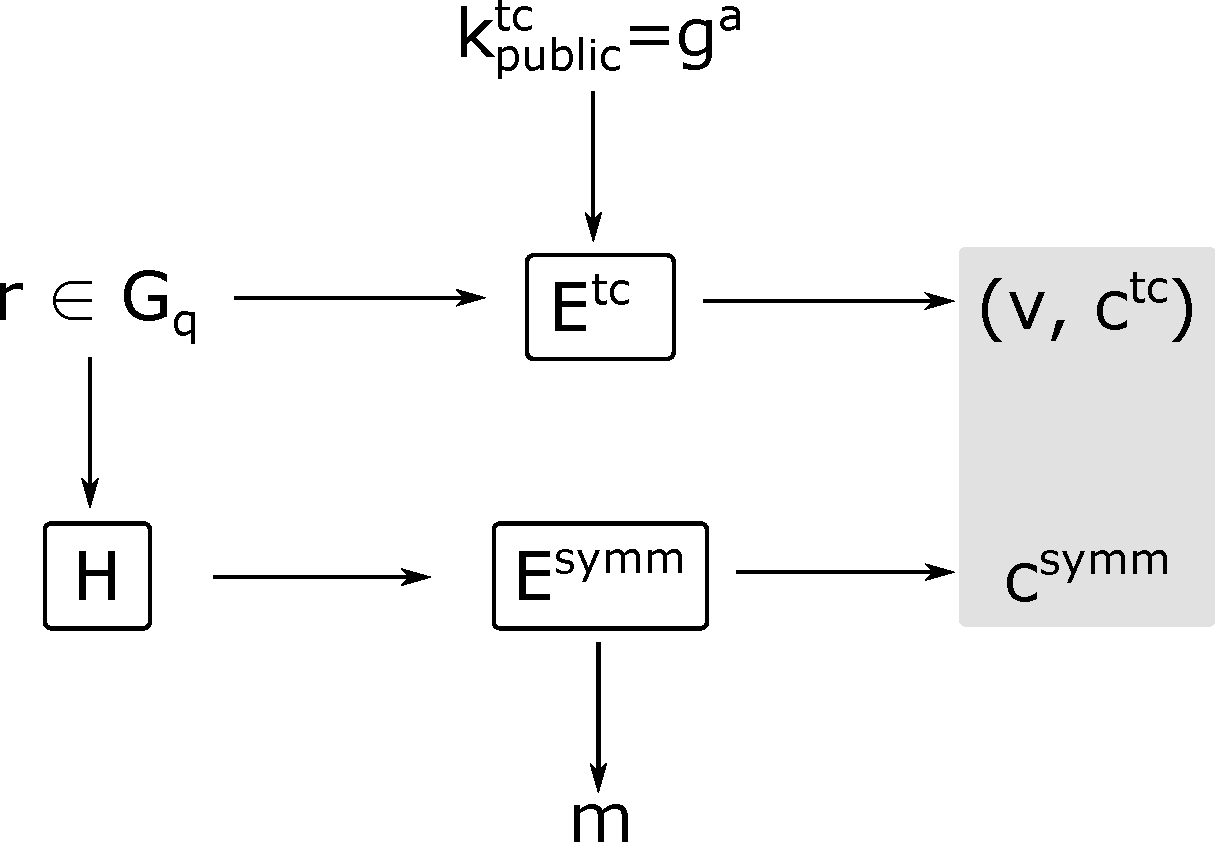
\includegraphics[width=0.4\textwidth]{dia/hybrid_scheme.pdf}
    \caption{Übersicht über das umgesetzte hybride Verschlüsselungsschema.}
    \label{fig:hybrid_scheme}
\end{figure}

\subsection{Service und Setup-Verfahren}

% Setup: Clients, KeyParameter, ThresholdParameter
% auf bereits in impl-pseudonymity geschriebenes zurückgreifen

Um die Parameter für das kryptographische Schwellwertschema setzen zu können, wurde die Konfigurationsoberfläche erweitert. Hier müssen nun Angaben zur Schlüsselstärke, zu beteiligten Teilnehmern und erforderlichen Anzahl an Teilnehmern für die Entschlüsselung eines Datenbankeintrages gemacht werden.

Anschließend können berechtigte Benutzer die Aufdeckung eines Pseudonyms über das Webinterface anfragen. Anschließend werden von den teilnehmenden Clients die partiellen Entschlüsselungen entgegengenommen. Liegen ausreichend partielle Verschlüsselungen vor, so werden diese mithilfe der Bibliothek kombiniert und damit der Halter des Pseudonyms entschlüsselt und aufgedeckt. 

\subsection{Client-Anwendung}

%- Shares empfangen und verschlüsselt abspeichern
%
%- Enthält Webserver um Shares niemals auf dem Server speichern zu müssen

Für Teilnehmer, die an dem Schwellwertschema beteiligt sind, wurde eine konsolenbasierte Anwendung entwickelt, die die folgende Funktionalität bereitstellt:

Clients melden sich zu Beginn an dem Pseudonym-Service an und können in der anschließenden Setup-Phase mit in das Verfahren integriert werden. Jeder teilnehmende Client empfängt nach der Generierung das für ihn bestimmte Share vom Server und speichert dieses verschlüsselt lokal ab. Hierzu enthält die Anwendung einen lokalen Webserver. Dies ermöglicht es dem Pseudonym-Service die \textit{Shares} nicht speichern und nach der Generierung sofort entfernen zu können. 

Anschließend können sich Teilnehmer regelmäßig nach neuen Anfragen zur Aufdeckung eines Pseudonyms erkundigen. Wurde eine neue Anfrage empfangen, so kann der Teilnehmen diese annehmen oder ablehnen. Die Annahme führt zur Berechnung einer partiellen Entschlüsselung mithilfe der Bibliotheksfunktion, die anschließend an den Pseudonym-Service gesendet wird.

\subsection{Proxy}

%- Empfängt PublicKey vom Service und nutzt ihn zur Nachrichtenverschlüsselung

Das im Syslog-Proxy implementierte Plugin zur Pseudonymisierung empfängt während der Initialisierung den während der Schlüsselerzeugung generierten öffentlichen Schlüssel vom Pseudonym-Service. Bei einer eintreffenden Syslog-Nachricht werden die zu pseudonymisierenden Daten mit diesem Schlüssel unter Nutzung der Bibliotheksfunktion verschlüsselt und zusammen mit den bereits in Abschnitt \ref{sec_impl_pseudonymity} beschriebenen weiteren Daten an den Service gesendet.